
\newpage
\section{Modeling with \henshin}
\label{sec:modeling}

% Stereotypes
\newcommand{\action}[1]{\ensuremath{\langle\!\langle\mathsf{#1}\rangle\!\rangle}}

\henshin~\cite{henshin,henshin-website} is a modeling language and toolset that implements the double-pushout approach~\cite{Corradini97} for attributed typed graph transformation, based on structural data model in the Eclipse Modeling Framework~\cite{EMF}. Due to lack of space, we describe the relevant concepts only informally here. A \emph{graph transformation system} (GTS) consists of (1)~an (attributed) type graph, (2)~a set of parameterized\footnote{For a formal definition of graph transformation systems with parameterized rules see, e.g.,~\cite{HGM06}.} transformation rules, and (3)~a graph representing the initial state. Figure~\ref{fig:railcab} depicts the type graph and two parameterized transformation rules for modeling the RailCab system~\cite{RailCab} in \henshin.

\begin{figure}[t!]
\centering
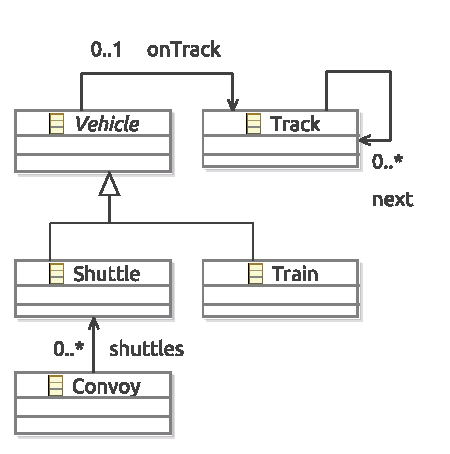
\includegraphics[width=4.7cm]{images/classes}\hspace{3mm}%
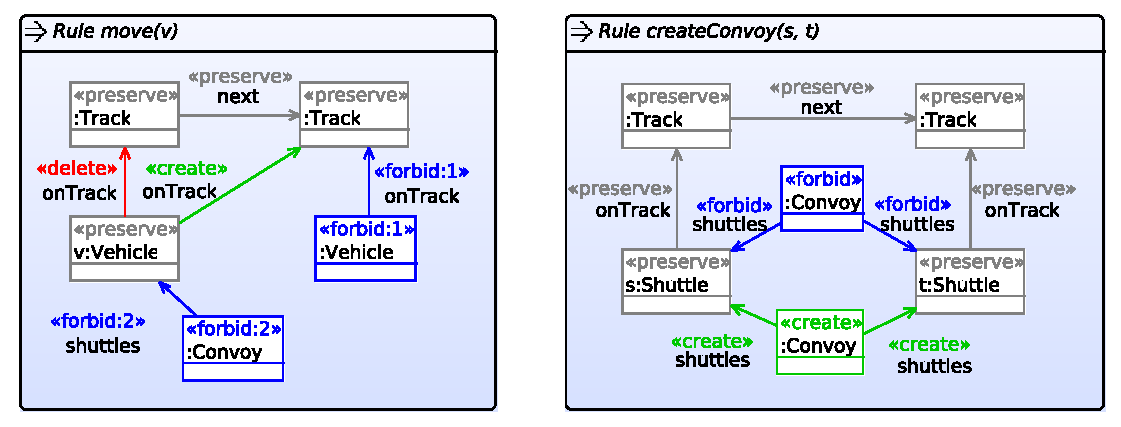
\includegraphics[width=11cm]{images/rules}
\vspace{-7mm}
\caption{Type graph (left) and transformation rules (mid and right) for the RailCab system in \henshin}
\label{fig:railcab}
\end{figure}

% System states in this approach are gioven by attributed typed graphs and the operational semantics is defined using parameterized graph rewrite rules..

\halflineup
\paragraph{(1) Type graph}
We distinguish five different node types: \textsf{Track}, \textsf{\textit{Vehicle}}, \textsf{Shuttle}, \textsf{Train} and \textsf{Convoy}. \textsf{\textit{Vehicle}} denotes an abstract node type and thus cannot be instantiated. \henshin supports node type inheritance which we use here to define \textsf{Shuttle} and \textsf{Train} as concrete realizations of \textsf{\textit{Vehicle}}. The edge type \textsf{next:Track}$\to$\textsf{Track} is used to model the topology of the railway system. The edge type \textsf{onTrack:\textit{Vehicle}}$\to$\textsf{Track} is used to specify the location of vehicles and \textsf{shuttles:Convoy}$\to$\textsf{Shuttle} models the existence of convoys between shuttles.

\definecolor{mygreen}{RGB}{0,200,0}
\definecolor{myred}{RGB}{200,0,0}
\definecolor{myblue}{RGB}{0,0,200}

\halflineup
\paragraph{(2) Parameterized transformation rules}
The parameterized transformation rules \textsf{\textit{move(v:Vehicle)}} and \textsf{\textit{createConvoy(s:Shuttle,t:Shuttle)}} in Figure~\ref{fig:railcab} are used here to model the operational semantics of the RailCab system. In the syntax of \henshin, rewrite patterns are denoted using the stereotypes \textcolor{darkgray}{\action{preserve}}, \textcolor{mygreen}{\action{create}}, \textcolor{myred}{\action{delete}} and \textcolor{myblue}{\action{forbid}}, respectively for matching and preserving, creating, deleting, and forbidding the existence of nodes or edges of a given type. The rule \textsf{\textit{move(v:Vehicle)}} moves the shuttle or train given by the parameter \textsf{\textit{v}} from its current track to one of its successor tracks. 
\begin{wrapfigure}{r}{3.3cm}
  \vspace{-5mm}
  \begin{center}
    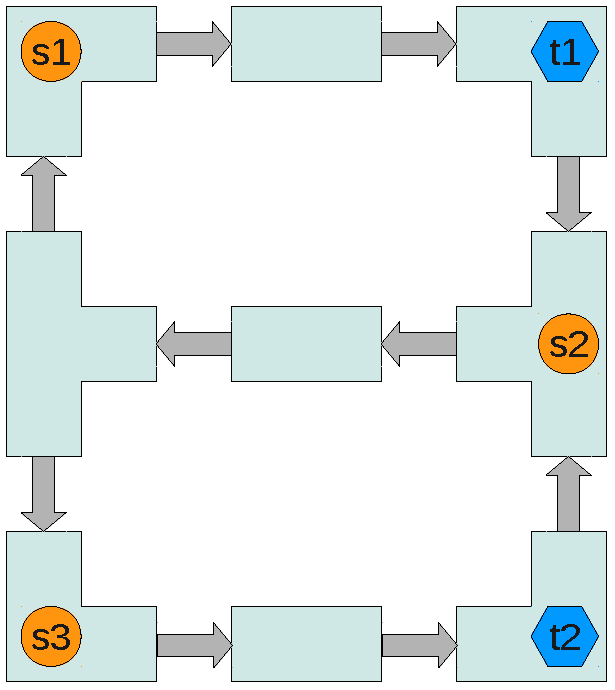
\includegraphics[width=3.25cm]{images/system}
  \end{center}
  \vspace{-5mm}
  \caption{Initial state}
  \label{fig:system}
  \vspace{-8mm}
\end{wrapfigure}
This is possible only if (1)~no other vehicle is on the next track, and (2)~the vehicle is currently not part of a convoy. The second constraint is added because modeling the movement of convoys is more involved and is for simplicity reasons not modeled here. The rule~\textsf{\textit{createConvoy(s:Shuttle,t:Shuttle)}} creates a convoy node between two shuttles which are located at adjacent tracks, if there is no convoy existing yet between them. We also introduce the rule~\textsf{\textit{deleteConvoy(s:Shuttle,t:Shuttle)}} which removes a convoy node again (not shown here).

\halflineup
\paragraph{(3) Initial state}
As initial state we use the typed traph which is schematically depicted in Figure~\ref{fig:system}. It consists of 9 interconnected tracks, 3 shuttles (depicted as circles) and 2 trains (depicted as hexagons) distributed on the tracks.

% A rule is a tuple $(r: L \rightharpoonup R)$
% A graph transformation system (GTS) is a pair $\langle P,G_0\rangle$ with $G_0$ an initial graph and $P$ a set of \emph{rules} of the form $p=\langle L,R,r,(C_i)_{i=1..n},(c_i)_{i=1..n}\rangle$ with $n\in \mathbb{N}$ where $L$ and $R$ are graphs called the left-hand side (LHS) and the right-hand side (RHS), $r : L \rightharpoonup R$ is a partial graph homomorphism, $\{C_i\}_{i=1..n}$ is a family of \emph{negative application conditions} (NACs) and $(c_i : L \to C_i)_{i=1..n}$ a family of total graph homomorphisms. For a graph $G$ a \emph{match} of a rule $p$ is a total graph homomorphism $m: L \to G$. Let $G'$ be the graph derived from $G$ by removing $m(L \setminus \mathit{dom}(r))$ and adding $R \setminus \mathit{codom}(r)$. Then $G \overset{r,m}{\Longrightarrow} G'$ is called a \emph{derivation}.

% \bigskip
% 
%  for NACs. Node inheritance: \textsf{Train} and \textsf{Shuttle} are specialization of the abstract type \textsf{Vehicle}. Graphical rule editor.
% High-level graphs: Structural data models\footnote{\ldots based on the Eclipse Modeling Framework}. Support for nested rules (amalgamation).
% 
% 
% Figure~\ref{fig:railcab} depicts two example rules for RailCab \cite{?}
% For simplicity, we do not model the movement of convoys. To avoid deadlocks, we also add a rule (note shown here) for removing a convoy again.
